\bghdr{images/fond-mac}

%\begin{center}
%
\includegraphics{images/logo_Mac}
%\end{center}



\subsection{Configuration sous Mac OS X}

La configuration est d\'etaill\'ee pour Mac OS 10.8 (\app{Mountain Lion}), elle est sensiblement identique sur Mac OS 10.9 (\app{Mavericks}),  Mac OS 10.7 (\app{Lion}), Mac OS 10.6 (\app{Snow Leopard}) et Mac OS 10.5 (\app{Leopard}).
Afin de conna\^itre la version que tu utilises, va dans le \menu{menu Pomme} puis s\'electionne \menu{\`A propos de ce Mac}.

\subsubsection{Configuration IP}

\flimage{images/mac_prefs_icone}{0.07}{l}
 \app{Pr\'ef\'erences R\'eseau}, accessible depuis l'article de menu \menu{Pr\'ef\'erences syst\`eme} du menu \menu{Pomme}, permet de configurer la connexion au r\'eseau. Par ailleurs, si au d\'emarrage un assistant te propose de configurer ton r\'eseau, refuse et utilise la proc\'edure du BR. En effet, le r\'eseau n\'ecessite une configuration particuli\`ere \`a l'X, plus complexe que celle effectu\'ee par cet assistant.


\noindent
  \begin{figure*}[h]
    \begin{center}  
     % \subfloat[Tiger]{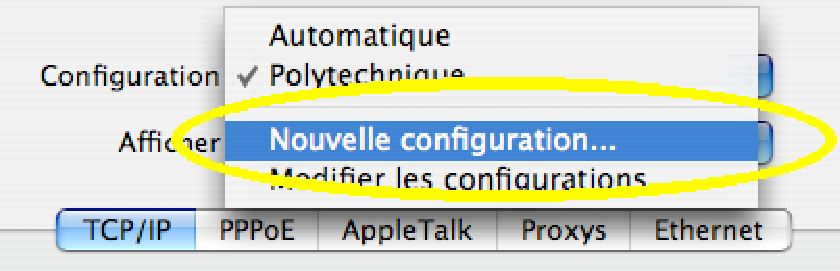
\includegraphics[width=0.47\textwidth]{images/mac_nouvelle_config} } 
     % \hfill
      \subfloat[Cr\'eer une nouvelle configuration r\'eseau]{ 
      \begin{minipage}{0.43 \textwidth}\begin{flushleft}
      {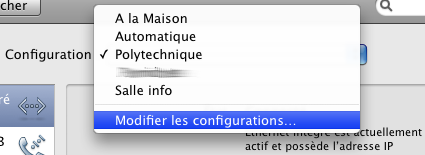
\includegraphics[width=0.96\textwidth]{images/mac_nouvelle_config_mountain_lion_1}}\\ \vspace*{2cm}
      {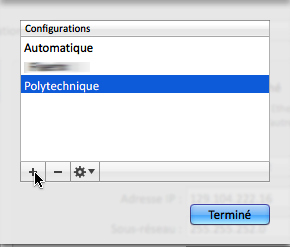
\includegraphics[width=0.96\textwidth]{images/mac_nouvelle_config_mountain_lion_2}} 
        \end{flushleft}  \end{minipage}
        }
        \subfloat[Configuration de l'interface r\'eseau \emph{Ethernet}, de l'adresse IP et du \emph{proxy}]{ 
        \begin{minipage}{0.43 \textwidth}\begin{flushright}
        {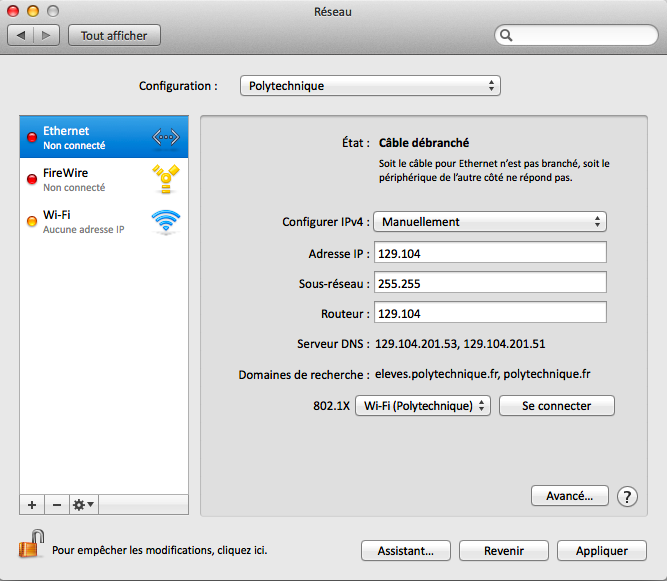
\includegraphics[width=0.96 \textwidth]{images/mac_config_ip_mountain_lion}} \\
        {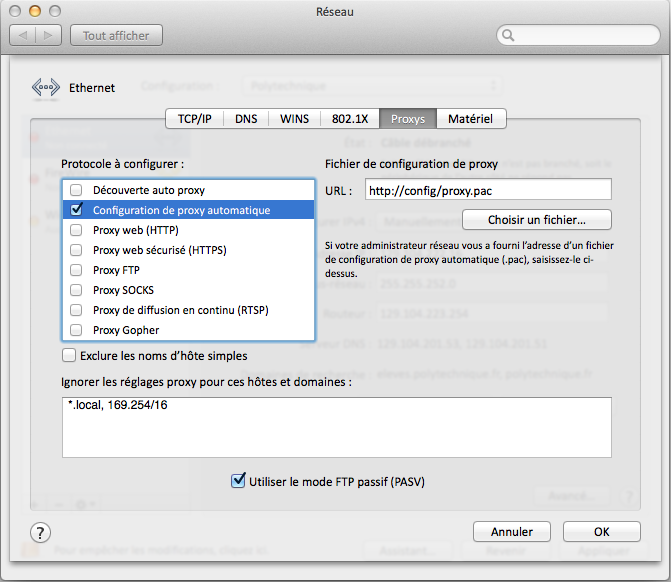
\includegraphics[width=0.96 \textwidth]{images/mac_config_proxy_mountain_lion}}
        \end{flushright}
        \end{minipage}
            \label{config:mac:ip:mountain_lion}   }
        \caption{Cr\'eer une nouvelle configuration r\'eseau}

    \end{center}
  \end{figure*}

%\pagebreak

La gestion des configurations r\'eseau de Mac OS X permet de cr\'eer plusieurs configurations et de passer en un clic de l'une  l'autre gr\^ace au sous-menu \menu{Configuration R\'eseau} du menu \menu{Pomme}. Cela est tr\`es pratique pour les machines vou\'ees \`a  \^etre connect\'ees \`a  plusieurs endroits successivement, typiquement les portables (voir la section \emph{Wi-Fi} page~\pageref{wifi} pour plus de pr\'ecisions sur le \emph{Wi-Fi}). Commence donc par cr\'eer une nouvelle configuration r\'eseau dans le menu d\'eroulant \menu{Configuration}.
\\
\\
Une fois la nouvelle configuration cr\'e\'ee, il faut configurer l'interface r\'eseau \emph{Ethernet}.


\app{Mountain Lion \& Mavericks} : Dans la colonne de gauche, s\'electionne \menu{Ethernet}.

Choisis alors \menu{Configurer IPv4} : \menu{Manuellement}. Tu trouveras toutes les valeurs d'adresses IP n\'ecessaires pour la configuration en page \pageref{calcul_ip} ou en te reportant aux captures d'\'ecran~\ref{config:mac:ip:mountain_lion}. Remplis le champ \emph{Routeur} avec l'adresse de passerelle que tu as calcul\'ee. Si une partie d'adresse IP est blanche sur ces captures, c'est qu'elle t'est personnelle et que tu dois la calculer !


  
  

%\imageref{images/mac_config_ip_leopard}{0.4}{Configuration IP (Leopard)}{!ht}{config:mac:ip:leopard}}
\vspace{4mm}

\textbf{Pour avoir acc\`es \`a  Internet, il faut aussi configurer le \emph{serveur DNS} et le \emph{proxy}.}

Configuration du \emph{serveur DNS} : clique sur le bouton \menu{Avanc\'e...} puis va dans l'onglet \menu{DNS}. Ajoute les serveurs DNS 129.104.201.53 et 129.104.201.51 dans la colonne de gauche et les domaines de recherche \emph{eleves.polytechnique.fr} et \emph{polytechnique.fr} dans la colonne de droite.



Configuration du \emph{proxy} : va dans l'onglet \menu{Proxys} et remplis l'URL comme dans la capture d'\'ecran. N'oublie pas d'activer le mode passif pour les transferts en FTP, en cochant la case comme dans la capture.

Sous Mac OS, le r\'eglage du proxy se fait au niveau des pr\'ef\'erences syst\`emes et n'a donc pas \`a \^etre sp\'ecifi\'e pour chaque navigateur. Tu peux donc sauter la partie \emph{Configuration de ton navigateur Web}.



%\subsubsection{Configuration antivirus}

%Bien qu'il soit important de maintenir ton syst\`eme \`a  jour, un antivirus est pour l'instant tout \`a  fait superflu sur Mac,
%puisqu'aucun virus fonctionnel n'a encore vu le jour. Attention cependant, n'ouvre pas des fichiers dont tu ne te sois pas assur\'e la provenance,
%et essaie de te tenir au courant des actualit\'es concernant les failles des applications que tu utilises.


% \subsubsection{Autres logiciels utiles}

%\flimage{images/mac_qrezix_icone}{0.07}{l} \app{qRezix} : en deux mots, c'est un programme d\'evelopp\'e par le BR pour faciliter la vie sur le r\'eseau. Tu peux le r\'ecup\'erer via le lien qRezix sur \server{Frankiz} ou sur \urllink{http://br.frankiz.net/qrezix/mac/}. Pour plus de d\'etails, voir le paragraphe consacr\'e \`a  qRezix \`a  la page \pageref{qrezix}. \\

%\app{Leopard} : le pare-feu se r\`egle pour chaque application; tu n'auras qu'\`a  r\'epondre \menu{Autoriser} lorsqu'il te demandera si tu veux \menu{Autoriser les connexions entrantes}.

%\noindent  \app{Tiger} : Attention, si ton \emph{firewall} est activ\'e, tu dois ouvrir les ports 5050, 5053 et 5055 en TCP. Pour cela va dans \app{Pr\'ef\'erences Syst\`eme}, dans le module \menu{S\'ecurit\'e}, onglet \menu{Coupe-feu}. S'il est \'ecrit \menu{Coupe-feu activ\'e}, clique le bouton \menu{Nouveau} et remplis la bo\^ite de dialogue comme sur la capture d'\'ecran ci-dessous pour ouvrir les ports.

%\imagepos{images/mac_firewall}{0.5}{Ouvrir les ports pour \app{qRezix} (Tiger)}{!ht}

%\flimage{images/mac_conversation_icone}{0.1}{l}
%\noindent\app{Colloquy}, un client IRC dans le m\^eme esprit qu'\app{iChat}. Il dispose d'une interface tr\`es simple ne n\'ecessitant pas de conna\^itre les commandes IRC. Tu peux te reporter \`a  la page \pageref{irc} pour plus d'infos sur l'IRC. \app{X-Chat Aqua} est un autre client IRC, plus riche en fonctionnalit\'es, mais moins agr\'eable \`a  utiliser. \\

%\flimage{images/mac_netnewswire_icone}{0.1}{l}
%\noindent\app{NetNewsWire} est la r\'ef\'erence des clients RSS sur Mac, et est maintenant gratuit. Dans le m\^eme genre, on peut citer \app{Vienna}, un client RSS open source, dont le d\'eveloppement actif est prometteur. Les flux RSS permettent d'agr\'eger dans un seul logiciel des informations en provenance de nombreux sites web, qui peuvent provenir de forums de discussions, de mises \`a  jour de logiciels, d'informations internationales\dots \\ \\

% \label{mac-fink}
% \flimage{images/mac_fink_icone}{0.07}{l} 
%  \app{Fink} est la mani\`ere la plus simple d'installer sur Mac OS X nombre de logiciels issus du monde Unix (Linux par exemple). Gr\^ace \`a  lui, tu pourras installer les m\^emes logiciels que dans les salles informatiques. Par exemple, tu pourras installer Scilab sans trop de peine\dots La configuration n\'ecessaire se trouve sur la page \urllink{https://br.binets.fr/Miroir\_Fink}.
% 
% \paragraph{}
% \flimage{images/logo_Windows}{0.1}{l}
%  \app{Windows et les Mac Intel} : Maintenant il est possible d'installer Windows gr\^ace \`a  \app{Boot Camp}, livr\'e avec \app{Leopard} et les version suivantes. Cela te permettra de profiter des quelques applications du monde PC qui valent le coup tout en gardant ton Mac. Tu peux \'egalement virtualiser Windows (utiliser Windows en utilisant en m\^eme temps Mac OS) gr\^ace \`a  \app{VMware Fusion}, \app{VirtualBox} ou \app{Parallels Desktop}. Le  d\'efaut de cette solution est que tu n'as pas d'acc\'el\'eration 3D, donc pour les jeux il te faudra red\'emarrer. Ces trois logiciels sont disponibles sur leurs sites \emph{web} respectifs. \`A toi de choisir !

\clearpage
